\section{Implementation}\label{sec:impl}
In this section, we elaborate on how we collect data for training, the specific parameters that we choose for two orthogonal neural networks, and system integration.

\paragraph{Data generation}
For each scene, we trained two independent neural networks: foveal and periphery. We sampled the rendered view for two networks accordingly. To train the foveal neural network, we rendered an image of resolution $256^2$ per 20 deg. For periphery neural network, we rendered an image of resolution $256^2$ per $60$ deg. We repeated the above every $5$ cm on each axis.
% \nothing{
%\paragraph{Input encoding}
Similar to \cite{mildenhall2020nerf}, we also extend the input dimensions ($d=3$) to a higher dimensional ($d=60$) for training. 
\nothing{This is achieved via coding the input as:
\begin{align}
\iota (p) = (\sin(2^0 p), \cos(2^0 p), ..., \sin(2^{L-1}p, \cos(2^{L-1}p))
\label{eqn:inputencode}
\end{align}
The function $\iota (\cdot)$ is applied to dimension of $\SpatialPt=(r_\SpatialPt,\theta_\SpatialPt, \phi_\SpatialPt)$.
In our experiment we choose $L=10$.\qisun{What is $L$?}\dnc{It's an encoding parameter for input. maps 3D input to $R^{6L}$ space, as \autoref{eqn:inputencode} shows}
}
\paragraph{Optimized network variables}
Following the optimization results from \Cref{sec:method:optimization}, we implemented both foveal and periphery neural network with $\mlpLayerNum=128$ and $\mlpChannelNum=4$ , and $\sphereNum = 32$ for foveal network and $\sphereNum = 16$ for periphery network. We will discuss the visual quality and performance difference in ~\Cref{sec:study:intra}. \nothing{We sampled the near foveal network and far foveal with $N_{sample}=16$ and $N_{sample}=16$, while we sampled the near ($1/distance < 0.5$) peripheral with $N_{sample}=8$,  $N_{channel}=64$,  $N_{layer}=4$ and far ($1/distance >= 0.5$) peripheral with $N_{sample}=8$,  $N_{channel}=128$,  $N_{layer}=4$.}
\nothing{
\dnc{Move to section 3.4 or just drop it (cause we have no detail analysis about the bound)? This small paragraph seems strange at here.}
\paragraph{Ray marching bounding}
For accelerating the performance and quality (as compared in \Cref{fig:method:bounding}), we bound the min/max of $\mathbf{\sphereRadius}$. The bounding range, together with $\sphereNum$, $\mlpLayerNum$ and $\mlpChannelNum$, are determined from a spatial-temporal optimization, as detailed in \Cref{sec:method:optimization}. %The bounding, however, may introduce subtle quality drop, as shown in \Cref{fig:method:bounding}.
\begin{figure}
    \centering
    \subfloat[w/o bounding]{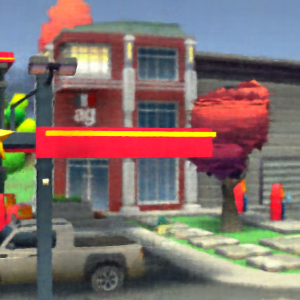
\includegraphics[width = 0.47\linewidth]{TOG/figs/depth_without_bound.png}}\hspace{1em}
    \subfloat[w bounding]{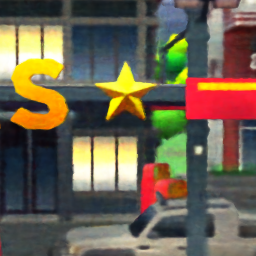
\includegraphics[width = 0.47\linewidth]{TOG/figs/depth_with_bound.png}}
    \Caption{Comparison of ray marching bounding.}
    {%
    }
    \label{fig:method:bounding}
\end{figure}
}%nothing
\paragraph{Integration} \dnc{this paragraph seems similar to 3.3.}
The stereoacuity significantly drops beyond fovea \cite{mochizuki2012magnitude}.
Our system reaches interactive performance (around 30FPS) for the first design -- the same procedure is applied to each eye (the details are addressed in \Cref{sec:study:intra}). To archive real-time performance (around 50FPS), we implemented mono-periphery for better performance. For each frame, we infer the same mid- and far- peripheral images for left and right eyes from the camera pose of central eye. In \Cref{sec:study:user}, we evaluated mono-periphery for subjective and objective measurements as well as discuss the visual quality and performance difference in ~\Cref{sec:study:intra}.
% \warning{We conducted a preliminary study to investigate how users perceive mono-periphery.}

\paragraph{Environment}
The system was implemented through OpenGL framework using CUDA and accelerated by TensorRT with Intel(R) Xeon(R) Gold 6230R CPU @ 2.10GHz (256GB RAM) and one NVIDIA GTX 3090 graphics card.
For each scene, we trained around 200 epochs for experiment use (about a day).